\chapter{Knot selection in spline models: cocaine dependence}
\label{applications-splines_knot_loc}
\chapterprecis{Yong Yi Lee, Theo Vos, Abraham D. Flaxman, Jed Blore, and Louisa Degenhardt}

For many conditions prevalence varies substantially as a function of
age.  Other epidemiological parameters, such as incidence and
excess mortality hazards, often have important age patterns as well.
The spline models introduced in chapter~\ref{theory-age_pattern_model}
provide a flexible framework for representing this age dependence.
However, some important modeling decisions are
necessary.  The following examples from estimating the
age-specific prevalence of cocaine dependence illustrate the
importance of choosing knot locations and smoothing levels
appropriately in a setting where the data speak relatively precisely
about the level and age pattern of the condition.

The American Psychiatric Association's \emph{Diagnostic and Statistical
Manual of Mental Disorders, Version IV,
Text Revision (DSM-IV-TR)} recognizes cocaine dependence as fulfilling $3$ or more of the
following $7$ dependence criteria during any time in the
same $12$-month period: \cite{american_psychiatric_association_diagnostic_2000, wagner_first_2002}
    \begin{itemize} \label{page:app-substance_dependence}
        \item tolerance to effects of cocaine (typically assessed
            by whether the same amount of cocaine has less effect or
            whether greater amounts are required to obtain the desired effect);
        \item withdrawal symptoms after use ceases;
        \item usage over longer period or in larger quantities than intended;
        \item persistent desire or unsuccessful efforts to control
          cocaine use;
        \item substantial time spent in obtaining, using, or recovering
          from effects of cocaine;
        \item reduction of important social, occupational, or recreational
          activities because of cocaine use;
        \item continued use despite knowledge of
          physiological or psychological problems induced by cocaine
          use.
    \end{itemize}

Despite a large body of data on cocaine \emph{use}, there are comparatively few
data available on the descriptive epidemiology of cocaine
\emph{dependence}.\cite{degenhardt_what_2011} Systematic review for cocaine
dependence identified $28$ prevalence data points,
covering $3$ GBD 2010 regions.  For this example, we have restricted our attention
to data from the USA (figure~\ref{fig:app-cocaine_data}).

    \begin{figure}[h]
        \begin{center}
            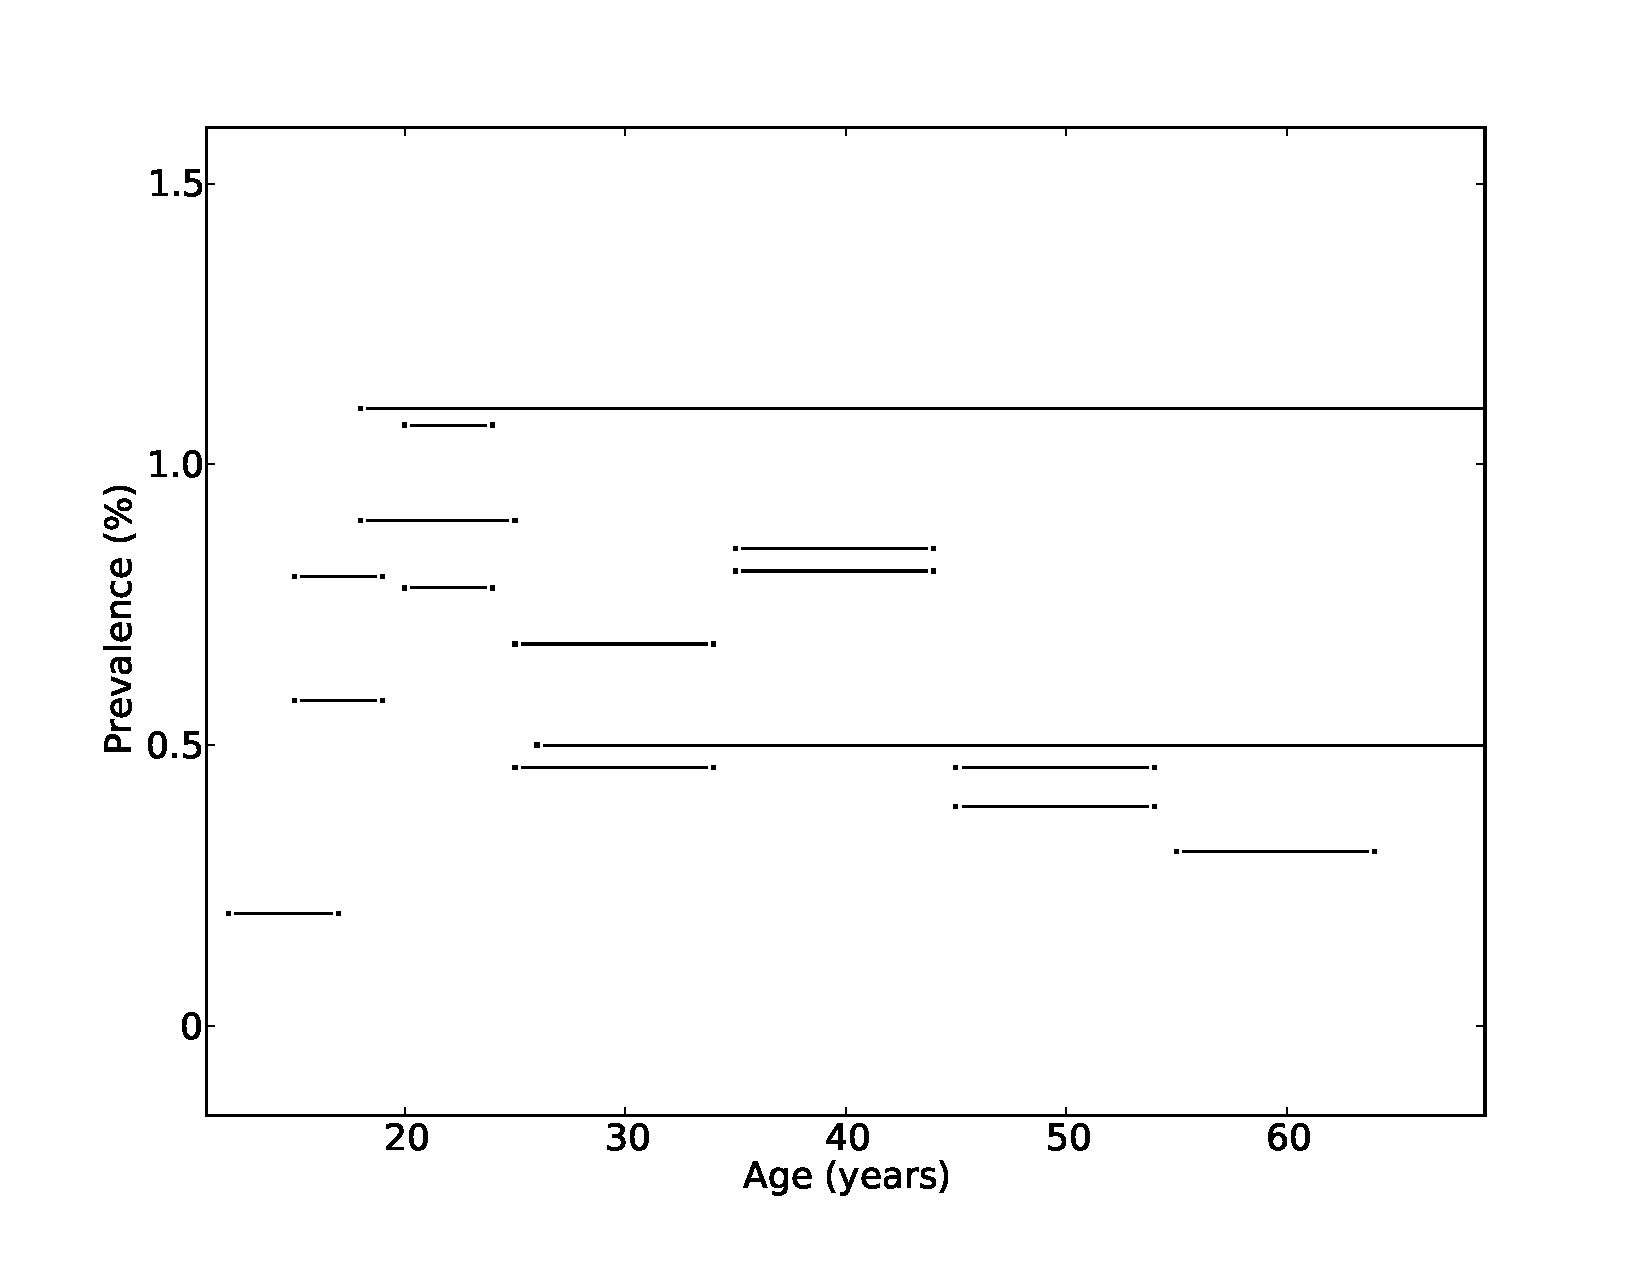
\includegraphics[width=\textwidth]{cocaine_dependence-data.pdf}
            \caption[Systematic review data for cocaine dependence.]{Prevalence
              data for cocaine dependence in the
              USA. Each horizontal bar represents
              a single data point extracted in systematic review.  The
              left and right endpoints indicate the start and end ages
              of the age interval for a data point, while the level of
              prevalence is represented by the distance of the bar
              above the $x$-axis.}
            \label{fig:app-cocaine_data}
        \end{center}
    \end{figure}

As discussed in chapter~\ref{theory-age_pattern_model}, we model
age-specific hazards with spline models.  In this
case, the spline model takes the form of a continuous, piecewise
linear function, with selected ``knots'' where the function is nonlinear.
These knots partition the age range
into intervals, and the choice of knots can be influential for the
resulting estimates.  In a setting where data are \emph{not} sparse and
noisy, estimates will not be very sensitive to the choice of knots.
However, when working with sparse and noisy data, the number and
location of knots are important decisions, as they can influence the
model results substantially.  Thus, the number of knots and locations
should be chosen a priori using expert knowledge concerning the
disease being modeled.  It is also
important to consider additional knots and alternative configurations
of knots as a sensitivity analysis.

To demonstrate the importance of the number of knots in a spline
model, we compare three models with differing numbers of knots in
figure~\ref{fig:app-cocaine_knots}.  The $7$-knot model for cocaine
dependence has knot set $\{15, 20, 25, 30, 40, 50, 65\}$, based on the theory that prevalence is $0$ in childhood,
changes rapidly during early adulthood, and then changes less rapidly
at older ages.  The age pattern of prevalence estimated with this
model is shown as a solid line with the $95\%$ highest posterior
density (HPD) shown as thin solid lines.

Another model we consider is a $4$-knot model, which has knots  set $\{15, 25,
40, 65\}$.  The estimates from this model, shown as a dotted line,
demonstrate how, seemingly paradoxically, fewer knots can lead to more
extreme estimates for certain ages.

We also fitted a model with $11$ knots, using knots spaced every $5$ years from
ages $15$ to $65$.
The estimates from this model are shown as a dashed line in
figure~\ref{fig:app-cocaine_knots}.  When data are sparse, adding
additional knots allows for estimates that follow the vagaries of the
data more closely, which may not be desired.  Smoothing priors for the
penalized spline model can address this.

    \begin{figure}[h]
        \begin{center}
            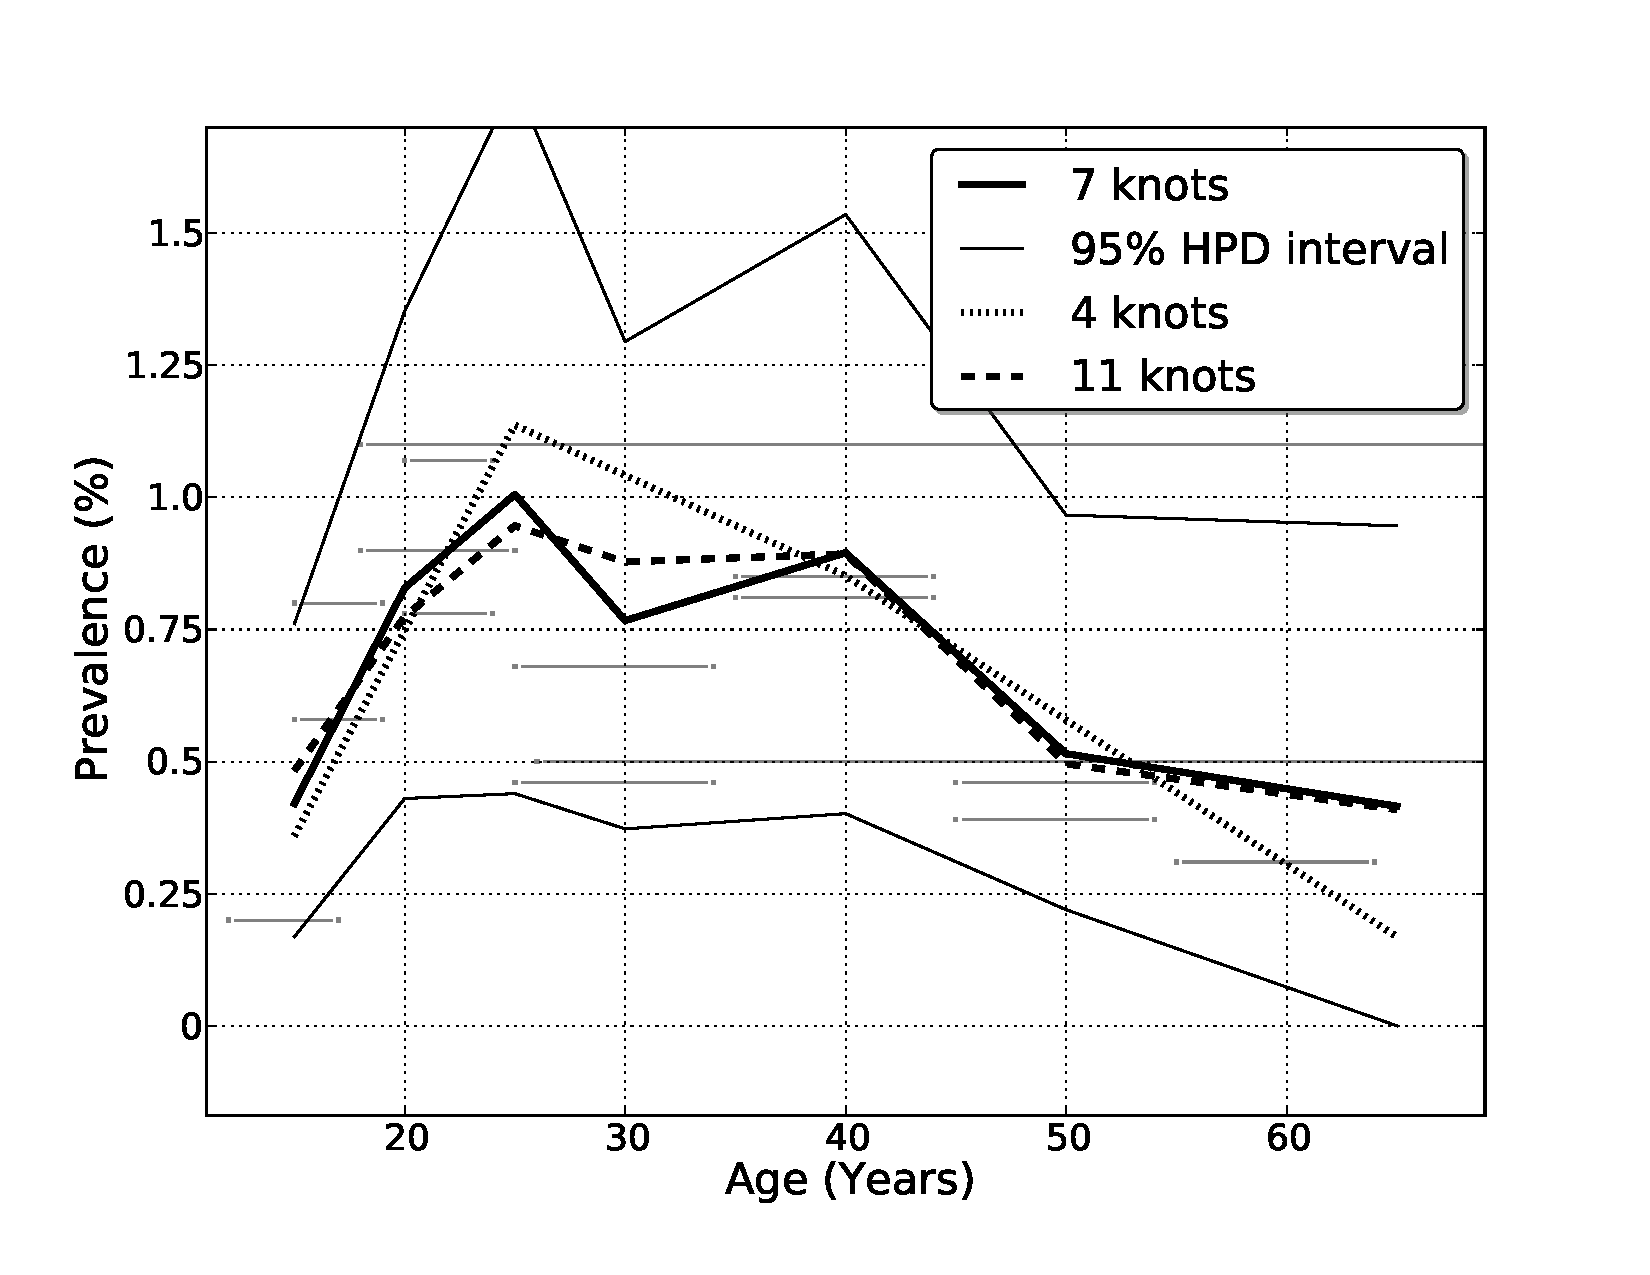
\includegraphics[width=\textwidth]{cocaine_dependence-knots.pdf}
            \caption[Prevalence estimates of cocaine dependence using spline
            models with varying numbers of knots.]{Prevalence estimates of cocaine dependence in the USA using a spline model with $4$, $7$, and $11$ knots. }
            \label{fig:app-cocaine_knots}
        \end{center}
    \end{figure}

The penalized spline model introduces an additional term to the model
prior to encode the belief that the age pattern is not too wiggly.
With the judicious choice of the smoothness hyperparameter, the model
can include more knots without using them to chase the noise around in
the noisy data.  The effects of four values of the smoothing parameter
are shown in figure~\ref{fig:app-cocaine_smoothing}.  The smaller the
parameter, the smoother the estimated age pattern and, hence, the less
influential the position of the knots.  However, too much smoothing
leads to overcompression of the prevalence estimates, resulting in
estimates that are not representative of the data.  If there were
enough time and data, it would be ideal to compare out-of-sample
predictive validity for a range of knots and smoothing parameters,
although in-sample goodness-of-fit statistics such as the Bayesian
information criteria (BIC) or deviance information criteria (DIC).

    \begin{figure}[h]
        \begin{center}
            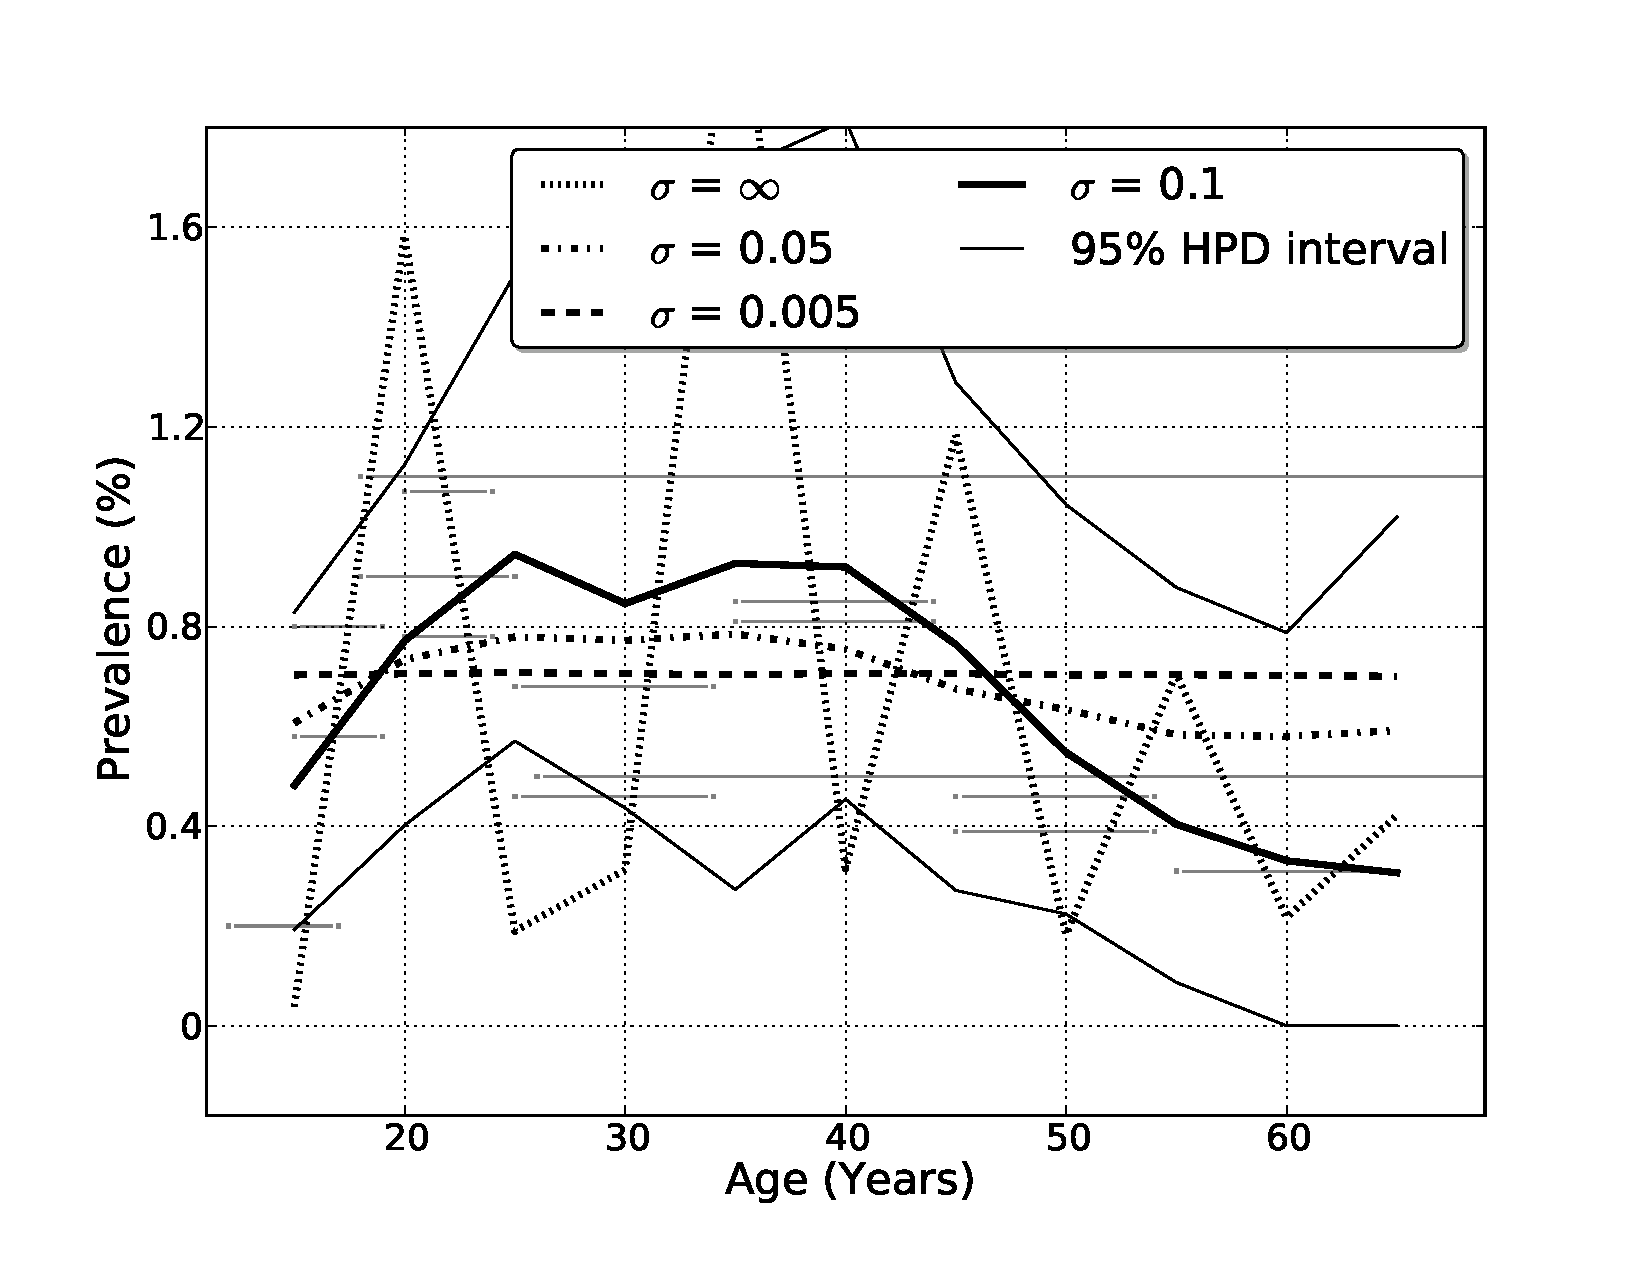
\includegraphics[width=\textwidth]{cocaine_dependence-smoothing.pdf}
            \caption[Prevalence estimates of cocaine dependence using a
              smoothing parameter.]{Prevalence estimates from the model
              with knots spaced every $5$ years
              using a penalized spline model with a smoothing
              parameter $\sigma$. }
        \label{fig:app-cocaine_smoothing}
        \end{center}
    \end{figure}

As shown by the figures, knot location and smoothing
hyperparameter selection can be influential parts of the model.
From the sensitivity analysis in figure~\ref{fig:app-cocaine_knots},
it appears that there is nothing to gain from adding additional
knots to the model, although it is possible to do so if an appropriate
smoothing parameter is included also.  In the next chapter, we will
consider a case where the data do not have such a clear story to
tell about the age pattern.
